\documentclass[11pt,a4paper]{article}
\usepackage[margin=2.2cm]{geometry}
\usepackage{booktabs}
\usepackage{array}
\usepackage{amsmath}
\usepackage{xcolor}
\usepackage{tikz}
\usepackage{pgfplots}
\pgfplotsset{compat=1.16}
\usepackage{float}
\setlength{\intextsep}{7pt}
\setlength{\textfloatsep}{7pt}
\usepackage{caption}
\captionsetup{font=small}
\usepackage[hidelinks]{hyperref}

% one colour per benchmark
\definecolor{cB1}{RGB}{31,119,180}
\definecolor{cB2}{RGB}{255,127,14}
\definecolor{cB3}{RGB}{44,160,44}
\definecolor{cB4}{RGB}{214,39,40}
\definecolor{cB5}{RGB}{148,103,189}
\definecolor{cB6}{RGB}{140,86,75}
\definecolor{cB7}{RGB}{227,119,194}
\definecolor{cB8}{RGB}{127,127,127}
\definecolor{cB9}{RGB}{188,189,34}
\definecolor{cB10}{RGB}{23,190,207}

\pgfplotsset{
  benchlines/.style={
    width=0.97\textwidth, height=7cm, grid=both, grid style={gray!20},
    tick label style={font=\small}, label style={font=\small},
    legend style={at={(0.5,1.02)}, anchor=south, legend columns=5, draw=none, font=\small},
    cycle list={
      {cB1,mark=*},{cB2,mark=square*},{cB3,mark=triangle*},{cB4,mark=diamond*},{cB5,mark=pentagon*},
      {cB6,mark=o},{cB7,mark=square},{cB8,mark=triangle},{cB9,mark=diamond},{cB10,mark=pentagon}},
    every axis plot/.append style={thick, mark size=1.6pt},
  },
  memx/.style={
    xmin=0.6, xmax=14.4, xtick={1,...,14},
    xticklabels={$2^{-1}$,$2^{-2}$,$2^{-3}$,$2^{-4}$,$2^{-5}$,$2^{-6}$,$2^{-7}$,$2^{-8}$,$2^{-9}$,$2^{-10}$,$2^{-11}$,$2^{-12}$,$2^{-13}$,$2^{-14}$},
    xlabel={Physical memory as a fraction of the virtual memory ($2^{-14}$ = 64 frames = 256\,KB)},
  },
}

\newcommand{\addbench}[1]{%
  \addplot table[x index=0, y=blender]{#1}; \addplot table[x index=0, y=fotonik3d]{#1};
  \addplot table[x index=0, y=gcc]{#1};     \addplot table[x index=0, y=imagick]{#1};
  \addplot table[x index=0, y=lbm]{#1};     \addplot table[x index=0, y=mcf]{#1};
  \addplot table[x index=0, y=perlbench]{#1}; \addplot table[x index=0, y=x264]{#1};
  \addplot table[x index=0, y=xalancbmk]{#1}; \addplot table[x index=0, y=xz]{#1};
  \legend{blender,fotonik3d,gcc,imagick,lbm,mcf,perlbench,x264,xalancbmk,xz}}

\begin{document}

\begin{titlepage}
\centering
\vspace*{1.2cm}
{\large\scshape Operating Systems Laboratory\par}
\vspace{0.3cm}
{\large Laboratory Assignment 4\par}
\vspace{2.4cm}
\rule{\textwidth}{1.2pt}\\[0.55cm]
{\Huge\bfseries Memory Management\par}
\vspace{0.35cm}
{\LARGE Page Tables, TLB and Page Replacement\par}
\vspace{0.55cm}
\rule{\textwidth}{1.2pt}
\vspace{2.6cm}

{\large\bfseries Submitted by\par}
\vspace{0.7cm}
{\large
\begin{tabular}{@{}lcl@{}}
Ayush Yadav       & \quad--\quad & CS24BT001\\[2mm]
Trisham Bepari    & \quad--\quad & CS24BT022\\
\end{tabular}\par}

\vfill
\begin{minipage}{0.88\textwidth}
\small
\noindent\textbf{Abstract.} A memory virtualization simulator was written in C\texttt{++} and run on
ten SPEC CPU 2017 benchmark traces of about 12 million memory references each. It models a single-level
page table, a two-level page table, a 128-entry LRU TLB and, finally, a physical memory smaller
than the virtual memory with LRU page replacement. A tiny fraction of the pages receives almost
all the references: the 1\,\% most used pages get 33--99\,\% of the accesses. The two-level page
table needs 14--171$\times$ less memory than the single-level one, and the TLB, with a 99.4--99.999\,\%
hit rate, halves the number of cycles and makes the extra level almost free. With physical memory
reduced from $\frac{1}{2}$ down to $\frac{1}{16384}$ of the virtual memory, no page is replaced
until memory is $\frac{1}{128}$ or smaller; after that the disk accesses dominate the cycle count
completely.
\end{minipage}
\vspace{1.2cm}

{\large \today\par}
\end{titlepage}

\section{Setup and Design}

\paragraph{Traces and system.} Each trace line is \texttt{<address>,<I/D>,<R/W>}. As specified,
only the lower 32 bits of the address are used, pages are 4\,KB, so a trace has
$2^{20}$ possible virtual pages (VPN $=(\text{address} \bmod 2^{32}) / 4096$). The ten traces have
11.5--12.9 million accesses each. All runs were done on an Intel Core i7-8665U (4 cores, 8
threads), Ubuntu with \texttt{g++ -O2}.

\paragraph{Programs.} There is one program per configuration, all with the same structure: read
the trace line by line, translate every access, add its cost, update the hash, and print the
statistics at the end.

\begin{table}[H]
\centering\small
\setlength{\tabcolsep}{5pt}
\begin{tabular}{@{}lll@{}}
\toprule
Program & Configuration & Cycles per access \\
\midrule
\texttt{part1}   & single-level page table          & 200 (page table) + 200 (data) = 400 \\
\texttt{part2}   & two-level page table             & 200 + 200 + 200 = 600 \\
\texttt{part3\_1} & single-level page table + TLB    & hit: 1 + 200 = 201, \quad miss: 1 + 400 = 401 \\
\texttt{part3\_2} & two-level page table + TLB       & hit: 201, \quad miss: 1 + 600 = 601 \\
\texttt{part4\_1}--\texttt{4\_4} & Parts I, II, III-1, III-2, limited memory & as above, $+\,2\times10^{7}$ per replacement \\
\bottomrule
\end{tabular}
\caption{Simulated configurations and their cost model.}
\label{tab:configs}
\end{table}

\paragraph{Frame allocation.} Frames are handed out in increasing order with one counter
\texttt{next\_free}: every frame below it is in use, every frame from it onward is free. Since
Parts I--III never free a frame, the counter is the whole free-frame manager and the first page
touched gets frame 0, the second frame 1, and so on. In Part IV, once \texttt{next\_free} reaches
the number of frames, a page fault takes the frame of the least recently used page instead.

\paragraph{Page tables.} The single-level table is an array of $2^{20}$ entries (4\,KB pages,
4 byte entries, so 4\,MB). The two-level table splits the VPN into a 10 bit outer index and a 10
bit inner index; inner tables of 1024 entries are allocated only when a page in their range is
first touched. Page table utilization is \emph{PT entries accessed / PT entries allocated}; for
the two-level table the accessed entries are the used outer entries (one per inner table) plus
the used inner entries.

\paragraph{TLB.} 128 entries, fully associative, LRU. Each entry stores the VPN, the frame and the
time of its last use; a VPN-indexed array tells in O(1) whether (and where) a page is in the TLB.
On a miss the entry with the oldest timestamp (or an empty one) is replaced.

\paragraph{Hash.} For every access, $H \leftarrow (H \oplus \text{frame}) \times 1099511628211
\bmod 2^{64}$ (FNV-1a style), starting from $H = 1469598103934665603$. The hash depends on the frame
of every access in order, so equal hashes mean two simulators produced exactly the same mapping.

\paragraph{Page replacement (Part IV).} Physical memory has
$\lfloor \text{fraction}\times 2^{20}\rfloor$ frames. Used frames are kept in a doubly linked list
ordered by last use (\texttt{std::list}; every access moves its frame to the front with
\texttt{splice}, in O(1)), so the LRU page is always at the back. A \emph{page fault} is an access to
a page that is not in memory. While there are free frames the fault is free (``the first set of
pages come for free''); otherwise the LRU page is evicted, its page-table entry is cleared, its
TLB entry (if any) is invalidated and $2\times10^{7}$ cycles are charged for the disk access. We
report the \emph{page fault rate} = page faults / accesses, and separately the number of
replacements, i.e.\ disk accesses.

\paragraph{Correctness checks.} (1) All four Part I--III programs give the same hash for every
benchmark (Table~\ref{tab:p12}). (2) With a large memory Part IV produces exactly the Part I hash,
since nothing is ever replaced. (3) The four Part IV programs give identical page faults,
replacements and hashes for every benchmark and memory size, as they must, because LRU does not
depend on the page table or TLB. (4) A separate, deliberately simple reference simulator (LRU memory
and TLB built from \texttt{std::list} and hash maps) was written and compared against all four
Part IV programs on all ten traces at eight memory sizes from 1 frame to $\frac{1}{2}$ of the
virtual memory: page faults, replacements, TLB hits and misses, cycles and hash matched in all
320 runs.

\paragraph{Building and running.} From \texttt{src/}; \texttt{filename} defaults to blender, the
\texttt{\_all} targets run every trace, the fraction can be a decimal or a ratio, and Parts I--III
also write the access count of every page to \texttt{results/}:
{\small
\begin{verbatim}
make all
make sim_part1 filename=gcc_memoryTrace.txt     # also part2, part3_1, part3_2
make sim_part1_all                              # every trace
make sim_part4_3 filename=gcc_memoryTrace.txt fraction=1/1024
make sim_part4_1_all fraction=0.25              # part4_1 to part4_4
\end{verbatim}}

\section{Part I: Single-Level Page Table}

\begin{table}[H]
\centering\small
\begin{tabular}{@{}lrrrrrr@{}}
\toprule
& & Frames & Cycles (I) & Cycles (II) & PT util. & PT util. \\
Benchmark & Accesses & used & $\times10^{9}$ & $\times10^{9}$ & single (\%) & two-level (\%) \\
\midrule
blender   & 12\,369\,560 &  1551 & 4.948 & 7.422 & 0.148 &  3.25 \\
fotonik3d & 12\,890\,021 &  1602 & 5.156 & 7.734 & 0.153 & 10.52 \\
gcc       & 12\,473\,306 &   990 & 4.989 & 7.484 & 0.094 &  1.46 \\
imagick   & 11\,548\,820 &    96 & 4.620 & 6.929 & 0.009 &  1.64 \\
lbm       & 12\,843\,431 &  2131 & 5.137 & 7.706 & 0.203 & 29.81 \\
mcf       & 12\,474\,523 &  1597 & 4.990 & 7.485 & 0.152 & 11.23 \\
perlbench & 12\,568\,037 &   630 & 5.027 & 7.541 & 0.060 &  1.35 \\
x264      & 11\,721\,344 &   234 & 4.689 & 7.033 & 0.022 &  1.99 \\
xalancbmk & 11\,972\,261 & 14\,325 & 4.789 & 7.183 & 1.366 & 25.53 \\
xz        & 11\,852\,222 &  8037 & 4.741 & 7.111 & 0.766 & 17.93 \\
\bottomrule
\end{tabular}
\caption{Parts I and II. Frames used equals the number of distinct pages. The hash is identical
in Parts I, II, III-1 and III-2 for every benchmark (e.g.\ gcc: 18412861333054507796).}
\label{tab:p12}
\end{table}

\paragraph{Frames and cycles.} The benchmarks touch only 96 (imagick) to 14\,325 (xalancbmk)
distinct pages, i.e.\ 0.4--56\,MB of the 4\,GB address space. Every access costs exactly 400
cycles, so the cycle count is just $400\times$ the number of accesses (4.6--5.2 billion).

\paragraph{Page table utilization} is tiny: at most 1.37\,\% (xalancbmk) and below 0.21\,\% for
eight of the ten benchmarks. The single-level table always allocates all $2^{20}$ entries (4\,MB)
while only a few hundred or thousand of them are ever used.

\paragraph{Hypothesis: a small fraction of the pages sees a large fraction of the accesses.}
Figure~\ref{fig:lorenz} sorts the pages of each benchmark from most to least accessed and plots the
share of all accesses that goes to the top $x$\,\% of the pages. The hypothesis is strongly
\emph{supported}. For every benchmark the top 1\,\% of the pages gets at least 33\,\% of the
accesses and for seven benchmarks more than 83\,\%. For six benchmarks fewer than 1\,\% of the
pages account for 90\,\% of the accesses, and xz needs only 0.10\,\% (8 of its 8037 pages). The
converse also holds: most pages are rarely used; in xz the less used half of the pages receives only
0.09\,\% of the accesses. gcc, perlbench, x264 and imagick are the most spread out, but even there
10--16\,\% of the pages cover 90\,\% of the accesses.

\begin{figure}[H]
\centering
\begin{tikzpicture}
\begin{axis}[benchlines, height=6.6cm, xmode=log, xmin=0.5, xmax=100, ymin=0, ymax=100,
  xtick={0.5,1,2,5,10,20,50,100}, xticklabels={0.5,1,2,5,10,20,50,100},
  xlabel={Most accessed pages (\% of the pages used by the benchmark, log scale)},
  ylabel={Share of all accesses (\%)}]
\addbench{data/p1_lorenz.dat}
\end{axis}
\end{tikzpicture}
\caption{Cumulative share of accesses received by the most accessed pages.}
\label{fig:lorenz}
\end{figure}

\begin{table}[H]
\centering\footnotesize
\setlength{\tabcolsep}{3pt}
\begin{tabular}{@{}lrrrrrrrrrr@{}}
\toprule
& blender & fotonik3d & gcc & imagick & lbm & mcf & perlbench & x264 & xalancbmk & xz \\
\midrule
\% of accesses to top 1\,\% of pages & 93.4 & 90.1 & 34.1 & 83.0 & 92.6 & 94.6 & 32.7 & 40.0 & 93.4 & 98.8 \\
\% of accesses to top 10\,\% of pages & 99.2 & 91.3 & 82.5 & 89.2 & 94.1 & 97.9 & 89.3 & 90.1 & 95.3 & 99.5 \\
\% of pages for 90\,\% of accesses & 0.58 & 0.50 & 15.0 & 15.6 & 0.14 & 0.38 & 10.6 & 10.3 & 0.05 & 0.10 \\
\bottomrule
\end{tabular}
\caption{How concentrated the accesses are.}
\label{tab:conc}
\end{table}

\section{Part II: Two-Level Page Table}

\begin{table}[H]
\centering\footnotesize
\setlength{\tabcolsep}{3.5pt}
\begin{tabular}{@{}lrrrrrrrrrr@{}}
\toprule
& blender & fotonik3d & gcc & imagick & lbm & mcf & perlbench & x264 & xalancbmk & xz \\
\midrule
Inner tables       & 47  & 14 & 70  & 5  & 6  & 13 & 48  & 11 & 54  & 43 \\
Page table (KB)    & 192 & 60 & 284 & 24 & 28 & 56 & 196 & 48 & 220 & 176 \\
Smaller than 4\,MB by & 21$\times$ & 68$\times$ & 14$\times$ & 171$\times$ & 146$\times$ & 73$\times$ & 21$\times$ & 85$\times$ & 19$\times$ & 23$\times$ \\
\bottomrule
\end{tabular}
\caption{Size of the two-level page table (1024 outer entries + 1024 entries per inner table).}
\label{tab:p2}
\end{table}

\paragraph{Space.} Only 5--70 of the 1024 inner tables are ever allocated, so the page table
shrinks from 4\,MB to 24--284\,KB, 14--171$\times$ less (Table~\ref{tab:p2}). Utilization goes up
accordingly to 1.4--30\,\% (Table~\ref{tab:p12}). It is still far from 100\,\% for gcc,
perlbench, imagick, x264 and blender: their pages are scattered over many 4\,MB regions (the range
covered by one inner table), and each inner table is only sparsely used. lbm and xalancbmk use
their inner tables best (30\,\% and 26\,\%), because their pages are packed into a few contiguous
regions.

\paragraph{Time.} The price is one more memory access per translation: 600 instead of 400 cycles,
50\,\% more for every benchmark.

\paragraph{Hash.} The hash is identical to Part I for all ten benchmarks. This is expected: the
page table structure only changes \emph{where} the mapping is stored, not \emph{which} frame a page
gets, and frames are still given out in order of first touch.

\section{Part III: Adding a TLB}

\begin{figure}[H]
\centering
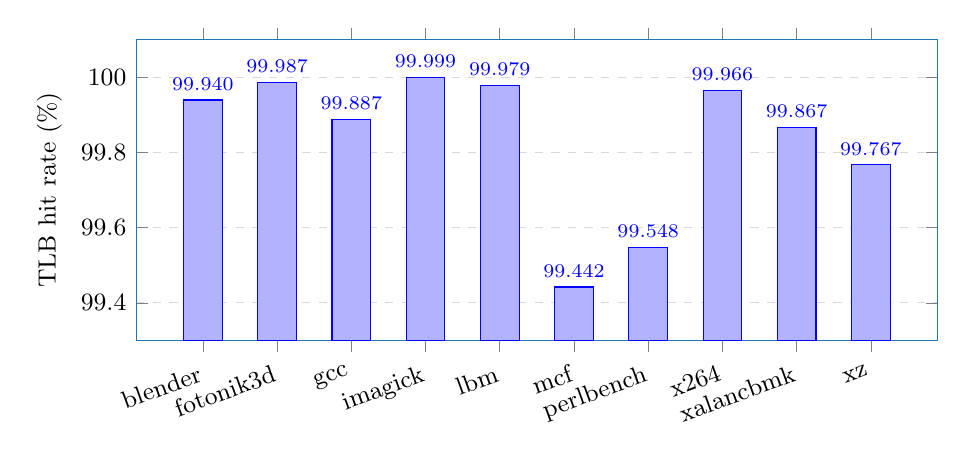
\begin{tikzpicture}
\begin{axis}[ybar, width=0.97\textwidth, height=5.4cm, bar width=14pt, ymin=99.3, ymax=100.1, ytick={99.4,99.6,99.8,100},
  symbolic x coords={blender,fotonik3d,gcc,imagick,lbm,mcf,perlbench,x264,xalancbmk,xz}, xtick=data,
  x tick label style={font=\small, rotate=20, anchor=north east}, tick label style={font=\small},
  ylabel={TLB hit rate (\%)}, label style={font=\small}, ymajorgrids, grid style={dashed,gray!30},
  nodes near coords, nodes near coords style={font=\scriptsize}, point meta=explicit symbolic, fill=cB1!70, draw=cB1]
\addplot coordinates {(blender,99.9398)[99.940] (fotonik3d,99.9867)[99.987] (gcc,99.8874)[99.887]
  (imagick,99.9992)[99.999] (lbm,99.9789)[99.979] (mcf,99.4421)[99.442] (perlbench,99.5484)[99.548]
  (x264,99.9659)[99.966] (xalancbmk,99.8673)[99.867] (xz,99.7669)[99.767]};
\end{axis}
\end{tikzpicture}
\caption{TLB hit rate (identical for the single-level and the two-level page table).}
\label{fig:tlb}
\end{figure}

\begin{table}[H]
\centering\small
\begin{tabular}{@{}lrrrrrr@{}}
\toprule
& TLB & Cycles (III-1) & Cycles (III-2) & III-1 vs I & III-2 vs II & III-2 vs III-1 \\
Benchmark & misses & $\times10^{9}$ & $\times10^{9}$ & (\% fewer) & (\% fewer) & (\% more) \\
\midrule
blender   &  7452 & 2.4878 & 2.4893 & 49.72 & 66.46 & 0.06 \\
fotonik3d &  1717 & 2.5912 & 2.5916 & 49.74 & 66.49 & 0.01 \\
gcc       & 14\,047 & 2.5099 & 2.5128 & 49.69 & 66.42 & 0.11 \\
imagick   &    96 & 2.3213 & 2.3214 & 49.75 & 66.50 & 0.00 \\
lbm       &  2704 & 2.5821 & 2.5826 & 49.74 & 66.49 & 0.02 \\
mcf       & 69\,597 & 2.5213 & 2.5352 & 49.47 & 66.13 & 0.55 \\
perlbench & 56\,759 & 2.5375 & 2.5489 & 49.52 & 66.20 & 0.45 \\
x264      &  3999 & 2.3568 & 2.3576 & 49.73 & 66.48 & 0.03 \\
xalancbmk & 15\,891 & 2.4096 & 2.4128 & 49.68 & 66.41 & 0.13 \\
xz        & 27\,631 & 2.3878 & 2.3933 & 49.63 & 66.34 & 0.23 \\
\bottomrule
\end{tabular}
\caption{Effect of the TLB on the number of cycles.}
\label{tab:p3}
\end{table}

\paragraph{Hit rate.} The TLB hit rate is at least 99.44\,\% (mcf) and reaches 99.9992\,\% for
imagick, whose 96 pages all fit in the 128 entries, so its only misses are the 96 first touches.
This follows directly from Part I: a handful of pages gets almost all the accesses, and 128
entries are enough to hold them. mcf and perlbench have the lowest hit rates: most of their accesses go to a few
pages too, but they keep coming back to a working set of a few hundred pages, more than the 128
entries (Part IV shows the same sets causing the most page faults).

\paragraph{Cycles.} With almost every translation coming from the TLB, an access costs 201
instead of 400 cycles, so the TLB removes 49.5--49.8\,\% of the cycles of Part I and 66.1--66.5\,\%
of Part II. The two-level page table, which cost 50\,\% extra in Part II, now costs at most
0.55\,\% extra (mcf), because its additional memory access is only paid on a TLB miss. Together,
the two techniques give the space saving of Part II at practically the speed of Part III-1.

\section{Part IV: Physical Memory Smaller than Virtual Memory}

Physical memory was halved repeatedly from $\frac{1}{2}$ to $\frac{1}{16384}$ of the virtual memory
(524\,288 down to 64 frames, 2\,GB down to 256\,KB). All four configurations were run at every size.

\begin{figure}[H]
\centering
\begin{tikzpicture}
\begin{axis}[benchlines, memx, ymode=log, height=7.2cm, ylabel={Page fault rate (\%, log scale)}]
\addbench{data/p4_faultrate.dat}
\end{axis}
\end{tikzpicture}
\caption{Page fault rate (page faults / accesses, including the first touch of every page).
Flat parts of a curve are compulsory faults only; no page is replaced there.}
\label{fig:faultrate}
\end{figure}

\begin{table}[H]
\centering\small
\setlength{\tabcolsep}{4pt}
\begin{tabular}{@{}l rrr rrr rrr@{}}
\toprule
& \multicolumn{3}{c}{$\frac{1}{1024}$ (1024 frames, 4\,MB)} & \multicolumn{3}{c}{$\frac{1}{4096}$ (256 frames, 1\,MB)} & \multicolumn{3}{c}{$\frac{1}{16384}$ (64 frames, 256\,KB)} \\
\cmidrule(lr){2-4}\cmidrule(lr){5-7}\cmidrule(l){8-10}
Benchmark & Faults & Replaced & Fault \% & Faults & Replaced & Fault \% & Faults & Replaced & Fault \% \\
\midrule
blender   &  1873 &   849 & 0.015 &  4710 &  4454 & 0.038 & 45\,752 & 45\,688 & 0.370 \\
fotonik3d &  1717 &   693 & 0.013 &  1717 &  1461 & 0.013 &   1717 &   1653 & 0.013 \\
gcc       &   990 &     0 & 0.008 &  4994 &  4738 & 0.040 & 39\,899 & 39\,835 & 0.320 \\
imagick   &    96 &     0 & 0.001 &    96 &     0 & 0.001 &   6559 &   6495 & 0.057 \\
lbm       &  2704 &  1680 & 0.021 &  2704 &  2448 & 0.021 &   2704 &   2640 & 0.021 \\
mcf       &  1638 &   614 & 0.013 & 40\,583 & 40\,327 & 0.325 & 87\,900 & 87\,836 & 0.705 \\
perlbench &   630 &     0 & 0.005 & 20\,365 & 20\,109 & 0.162 & 114\,375 & 114\,311 & 0.910 \\
x264      &   234 &     0 & 0.002 &   234 &     0 & 0.002 &   6319 &   6255 & 0.054 \\
xalancbmk & 14\,974 & 13\,950 & 0.125 & 14\,992 & 14\,736 & 0.125 & 16\,537 & 16\,473 & 0.138 \\
xz        & 15\,527 & 14\,503 & 0.131 & 24\,048 & 23\,792 & 0.203 & 32\,937 & 32\,873 & 0.278 \\
\bottomrule
\end{tabular}
\caption{Page faults, replacements (disk accesses) and page fault rate at three memory sizes.}
\label{tab:p4}
\end{table}

\paragraph{When does replacement start?} With the sizes suggested in the assignment
($\frac{1}{2}$, $\frac{1}{4}$, \dots) nothing at all is replaced: every benchmark uses at most
14\,325 pages, which fit as long as memory is at least $\frac{1}{64}$ of the virtual memory
(16\,384 frames). The first replacements appear at $\frac{1}{128}$ for xalancbmk, $\frac{1}{256}$ for
xz, $\frac{1}{512}$ for lbm, $\frac{1}{1024}$ for blender, fotonik3d and mcf, $\frac{1}{2048}$ for gcc
and perlbench, $\frac{1}{8192}$ for x264 and only at $\frac{1}{16384}$ for imagick (64 frames for
96 pages). Above these points the fault rate is only the compulsory rate, 0.001--0.12\,\%.

\paragraph{How fast do faults grow?} Thanks to the strong locality of Part I, the fault rate stays
low even when memory holds only a small fraction of the pages: at 64 frames it is between 0.013\,\%
and 0.91\,\%. The benchmarks behave very differently though. perlbench and mcf degrade the most
(0.91\,\% and 0.70\,\% at 64 frames): their hot set is a few hundred pages, and once that does not
fit every miss evicts a page that is needed again soon. fotonik3d and lbm hardly change at all:
below $\frac{1}{1024}$ their fault count stays at 1717 and 2704, exactly their TLB miss counts from
Part III. These programs work on a few pages at a time and do not come back to a page until much
later, so a page that leaves the TLB is not needed again for a long time, and extra memory beyond
a few dozen frames does not help them. For xalancbmk the jump comes immediately at
$\frac{1}{128}$, after which it stays almost flat: its many lightly used pages are the ones being
replaced, and they are rarely accessed again.

\begin{figure}[H]
\centering
\begin{tikzpicture}
\begin{axis}[benchlines, memx, ymode=log, height=7.2cm, ylabel={Cycles ($\times10^{9}$, log scale)}]
\addbench{data/p4_cycles_v3.dat}
\end{axis}
\end{tikzpicture}
\caption{Total cycles with the single-level page table and the TLB (\texttt{part4\_3}).}
\label{fig:cycles}
\end{figure}

\paragraph{Cycles.} A replacement costs $2\times10^{7}$ cycles, as much as 100\,000 TLB hits, so
the disk dominates as soon as a few replacements happen (Figure~\ref{fig:cycles}). gcc needs
$2.51\times10^{9}$ cycles with enough memory, but $9.7\times10^{10}$ at $\frac{1}{4096}$
($39\times$ more) because of 4738 replacements, and perlbench at 64 frames needs
$2.29\times10^{12}$ cycles, about $900\times$ more than in Part III. Once that happens the page
table structure and the TLB no longer matter: at $\frac{1}{4096}$, gcc takes 99.7, 102.2, 97.3
and $97.3\times10^{9}$ cycles with \texttt{part4\_1} to \texttt{part4\_4}, and the difference
between them is the same $2.5\times10^{9}$ cycles by which they differ in Parts I--III.

\paragraph{Effect on the TLB.} A replaced page has its TLB entry removed. As long as memory has
more frames than the TLB has entries, the replaced (least recently used) page is never in the TLB,
so the hit rate is exactly that of Part III. At 64 frames, fewer than the 128 TLB entries, the TLB
can hold pages that are no longer in memory, and these entries have to be invalidated: the hit rate
falls, for example from 99.94\,\% to 99.63\,\% for blender and from 99.55\,\% to 99.09\,\% for
perlbench.

\section{Part V: Simulation Time}

\begin{table}[H]
\centering\small
\begin{tabular}{@{}lrrrrrrrr@{}}
\toprule
Benchmark & part1 & part2 & part3\_1 & part3\_2 & part4\_1 & part4\_2 & part4\_3 & part4\_4 \\
\midrule
blender   & 0.73 & 0.76 & 0.72 & 0.77 & 0.76 & 0.77 & 0.78 & 0.76 \\
fotonik3d & 0.77 & 0.81 & 0.77 & 0.80 & 0.81 & 0.81 & 0.80 & 0.78 \\
gcc       & 0.74 & 0.76 & 0.74 & 0.77 & 0.77 & 0.77 & 0.76 & 0.75 \\
imagick   & 0.64 & 0.67 & 0.64 & 0.68 & 0.67 & 0.66 & 0.67 & 0.67 \\
lbm       & 0.81 & 0.83 & 0.79 & 0.81 & 0.81 & 0.81 & 0.80 & 0.80 \\
mcf       & 0.74 & 0.77 & 0.75 & 0.79 & 0.76 & 0.79 & 0.77 & 0.79 \\
perlbench & 0.76 & 0.78 & 0.75 & 0.79 & 0.76 & 0.78 & 0.77 & 0.81 \\
x264      & 0.67 & 0.71 & 0.68 & 0.70 & 0.69 & 0.70 & 0.70 & 0.70 \\
xalancbmk & 0.70 & 0.69 & 0.69 & 0.72 & 0.68 & 0.73 & 0.72 & 0.69 \\
xz        & 0.72 & 0.73 & 0.73 & 0.74 & 0.70 & 0.73 & 0.71 & 0.74 \\
\bottomrule
\end{tabular}
\caption{Simulation time in seconds (wall clock measured inside the program, median of 3 runs;
Part IV at $\frac{1}{1024}$). Times include reading the trace and, for Parts I--III, writing the
page count file.}
\label{tab:time}
\end{table}

Every simulator processes a benchmark in 0.64--0.83\,s, i.e.\ about 60\,ns per access, and the
eight programs differ by less than 10\,\%. The time is dominated by reading and parsing the
140--176\,MB text trace with \texttt{getline} and \texttt{atoll}: a program that only reads and
parses the gcc trace, without simulating anything, already takes 0.66--0.71\,s of the 0.72\,s that
\texttt{part1} needs. The page table walk, the TLB search over 128 entries (only on the rare
misses) and the LRU list update add very little on top. A faster simulator would therefore have
to start with the input, for example by mapping the file into memory and parsing the digits
directly, rather than with the simulation itself.

\section{Conclusion}

Memory references are highly concentrated: about 1\,\% of the pages receive most of the accesses.
This one fact explains all the other results. A single-level page table wastes almost all of its
4\,MB; a two-level table allocates only the regions in use and is 14--171$\times$ smaller, at the
cost of 50\,\% more cycles. A 128-entry TLB catches 99.4--99.999\,\% of the translations, which
halves the number of cycles and makes the second page table level almost free. Finally, with
LRU replacement the programs keep running with low fault rates even with a few hundred frames, but
since a disk access is $10^{5}$ times more expensive than a TLB hit, every replacement shows up
directly in the total cycle count, and the choice of page table or TLB becomes irrelevant compared
to the amount of physical memory.

\end{document}
